%%%%%%%%%%%%%%%%%%%%%%%%%%%%%%%%%%%%%%%%%%%%%%%%%%%%%%%%%%%%%%%%%%%%%%%%%%%%%%%%%%%%%%%%%%%%%%%%%%%
% Appendix -> Supplementary Tables and Figures of MOJITOO
% Author: Mingbo Cheng
%%%%%%%%%%%%%%%%%%%%%%%%%%%%%%%%%%%%%%%%%%%%%%%%%%%%%%%%%%%%%%%%%%%%%%%%%%%%%%%%%%%%%%%%%%%%%%%%%%%
\chapter{Appendix A: MOJITOO}
\label{chapter:appendixA}


\setstretch{1}

\graphicspath{{appendix/figs}}


\begin{table*}[ht]
\centering
\caption[Feature characteristics of 6 mulitmodal data]{Number of features, zero features, and different non-zero features statistic of 6 single cell mulitmodal data.}
\begin{tabular}{llrr} 
  \toprule & 
  \rotatebox{60}{Modality} & 
  \rotatebox{60}{\#features} & 
  \rotatebox{60}{feature =0 $(\%)$} \\
 dataset & & &\\
\midrule
\multirow{3}{*}{\shortstack[l]{tea}}
 & RNA & 36,601 & 97.05 \\ 
 & ATAC & 128,853 & 98.02 \\ 
 & ADT & 47 & 18.54 \\
\midrule
\multirow{3}{*}{\shortstack[l]{dogma}}
& RNA & 36,495 & 94.01 \\
& ATAC & 68,963 & 92.48\\
& ADT & 210 & 45.61\\
\midrule
\multirow{2}{*}{\shortstack[l]{skin}}
& RNA & 23,296 & 97.24 \\
& ATAC & 344,592 & 98.83\\
\midrule
\multirow{2}{*}{\shortstack[l]{pbmc}}
& RNA & 36,601 & 94.56\\
& ATAC & 108,377 & 93.35\\
\midrule
\multirow{2}{*}{\shortstack[l]{cite\_bm}}
& RNA & 17,009 & 94.79\\
& ADT & 25 & 0.48\\
\midrule
\multirow{2}{*}{\shortstack[l]{cite\_lung}}
& RNA & 33,514 & 98.32\\
& ADT & 52 & 17.19\\
\bottomrule \end{tabular}
\label{tab:multimodal_feature_statistic}
\end{table*}

\begin{table*}[ht]
\centering
\caption[Time consumption of MOJITOO]{Benchmarking experiments on SKIN-SHARE data set (time elapsed in minutes). Of note LIGER could only be executed with up to 28,147 cells. We also include  two versions of MOFA with the full input matrices (MOFA full) or with reduced input matrices (MOFA).}
\begin{tabular}{r|rrrrrrrrr}
  \hline
 cells & DIABLO & LIGER & MOFA-Full & MOFA & MOJITOO & scAI & schema & Symph-Int & WNN \\ 
  \hline
3000 & 2.00 & 0.65 & 1.65 & 0.46 & 0.42 & 5.69 & 2.12 & 0.46 & 0.51 \\ 
  6,000 & 6.91 & 1.06 & 3.10 & 0.88 & 0.63 & 15.29 & 4.10 & 0.78 & 0.82 \\ 
  9,000 & 13.33 & 1.63 & 4.58 & 1.14 & 0.88 & 33.37 & 4.84 & 1.10 & 1.17 \\ 
  12,000 & 21.18 & 2.19 & 7.24 & 1.31 & 1.13 & 62.68 & 5.70 & 1.30 & 1.56 \\ 
  15,000 & 28.52 & 2.59 & 11.20 & 1.60 & 1.37 & 121.74 & 6.98 & 1.59 & 1.92 \\ 
  18,000 & 40.85 & 3.02 & 18.53 & 2.26 & 1.83 & 171.82 & 8.02 & 2.09 & 2.50 \\ 
  21,000 & 53.88 & 3.61 & 34.51 & 2.58 & 2.08 & 249.61 & 9.08 & 2.43 & 2.90 \\ 
  24,000 & 69.14 & 4.23 & 43.96 & 2.85 & 2.30 & 350.98 & 10.56 & 2.64 & 3.26 \\ 
  27,000 & 89.49 & 4.58 & 52.47 & 3.19 & 2.56 & 485.13 & 11.79 & 2.95 & 3.68 \\ 
  30,000 & 103.26 & - & 67.53 & 3.21 & 2.48 & 637.52 & 13.09 & 3.01 & 3.74 \\ 
   \hline
\end{tabular}
\label{tab:time}
\end{table*}


\begin{table*}[ht]
\centering
\caption[Peak Memory of MOJITOO]{Peak memory consumption in gigabytes. Of note, LIGER could only be executed with up to 28,147 cells. We also include  two versions of MOFA with the full input matrices (MOFA full) or with reduced input matrices (MOFA)}
\begin{tabular}{r|rrrrrrrrr}
  \hline
 cells & DIABLO & LIGER & MOFA-Full & MOFA & MOJITOO & scAI & Schema & Symph-Int & WNN \\ 
  \hline
  3,000 & 9.61 & 10.88 & 1.66 & 3.20 & 1.61 & 6.27 & 10.66 & 3.19 & 1.61 \\ 
  6,000 & 10.87 & 9.99 & 2.37 & 4.76 & 2.11 & 10.65 & 11.41 & 4.74 & 2.11 \\ 
  9,000 & 15.25 & 9.09 & 2.51 & 6.37 & 2.46 & 10.32 & 11.66 & 6.34 & 2.46 \\ 
  12,000 & 20.34 & 12.90 & 3.90 & 7.95 & 3.28 & 14.26 & 11.68 & 7.91 & 2.89 \\ 
  15,000 & 20.38 & 12.04 & 4.42 & 9.56 & 3.43 & 20.22 & 12.07 & 9.51 & 3.88 \\ 
  18,000 & 35.06 & 16.80 & 6.58 & 9.09 & 4.31 & 26.36 & 12.39 & 9.09 & 4.09 \\ 
  21,000 & 42.29 & 15.92 & 9.17 & 9.28 & 5.01 & 34.14 & 13.11 & 9.28 & 5.58 \\ 
  24,000 & 50.61 & 21.85 & 12.49 & 8.86 & 4.85 & 43.27 & 13.29 & 8.86 & 5.84 \\ 
  27,000 & 57.22 & 20.93 & 17.94 & 13.05 & 5.94 & 58.91 & 13.74 & 13.05 & 5.93 \\
  30,000 & 78.30 & - & 22.47 & 13.09 & 6.34 & 75.92 & 14.28 & 13.09 & 6.79 \\ 
   \hline
\end{tabular}
\label{tab:memory}
\end{table*}


\begin{figure}[!ht]
  \centering
  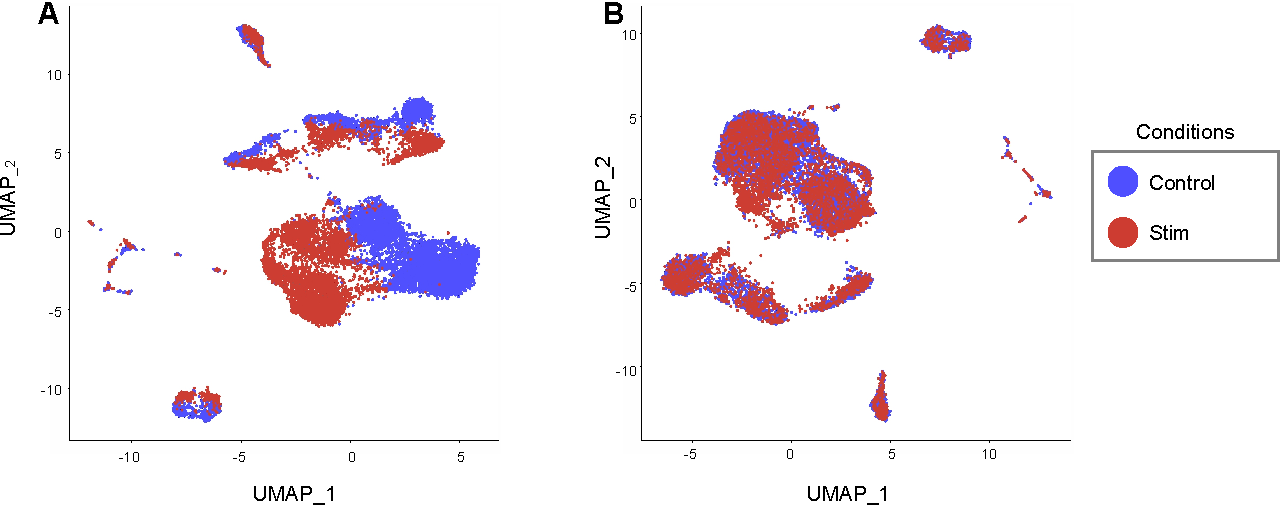
\includegraphics[width=0.95\textwidth]{batch_correction/fig}
  \vspace{0.1cm}
  \caption[With or without batch correction integration.]{\textbf{With or without batch correction integration}.}
  \label{fig:batch_correction}
\end{figure}

\begin{figure}[!ht]
  \centering
  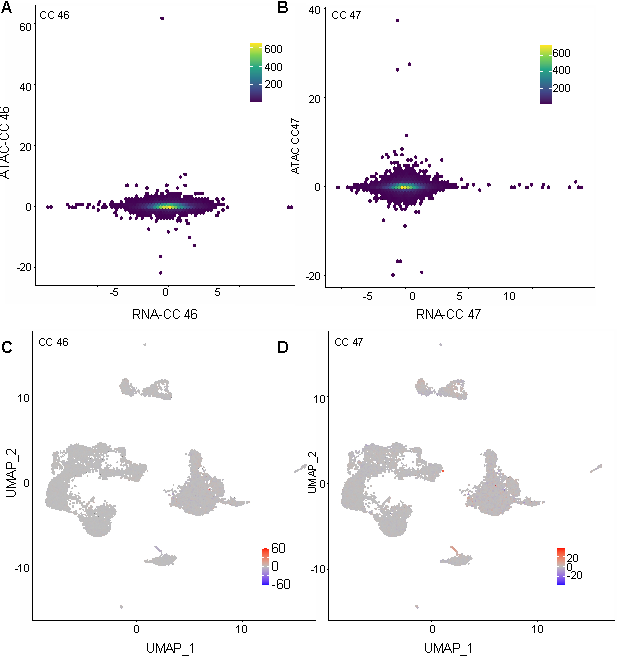
\includegraphics[width=0.95\textwidth]{CC_corrlations_last/fig}
  \vspace{0.1cm}
  \caption[Irrelevant components from CCA.]{\textbf{Irrelevant components from CCA.}.}
  \label{fig:CC_corrlations_last}
\end{figure}

\begin{figure}[!ht]
  \centering
  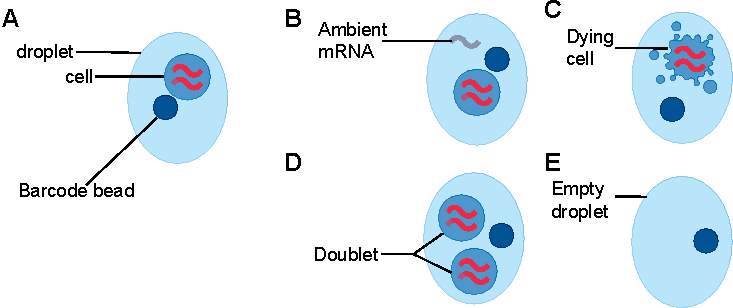
\includegraphics[width=0.95\textwidth]{Inte_UMAP/fig}
  \vspace{0.1cm}
  \caption[UMAP of multimodal integrated from 5 datasets.]{UMAP of multimodal integrated from 5 datasets.}
  \label{fig:UMAP_Integrated5}
\end{figure}


\begin{figure}[!ht]
  \centering
  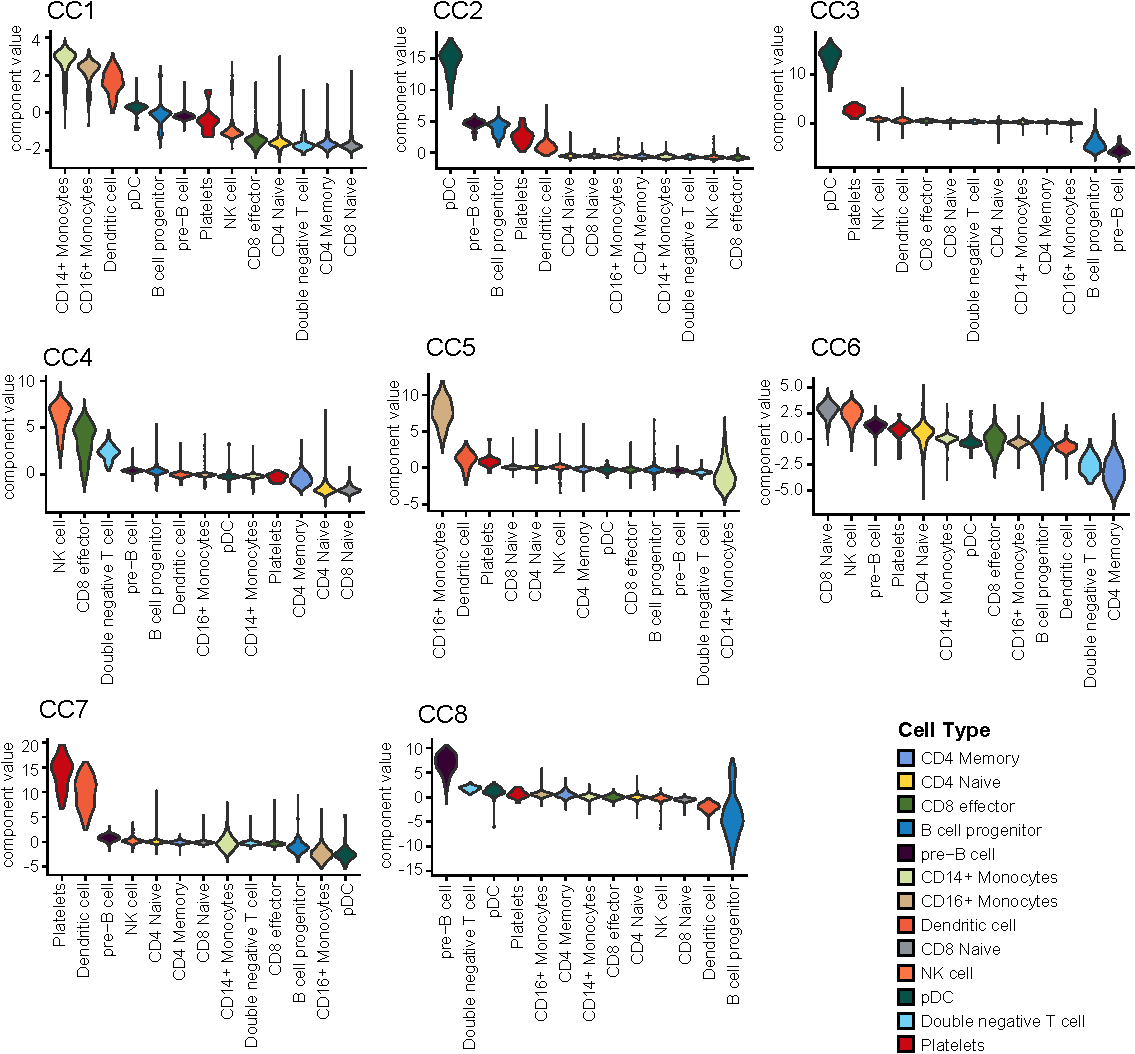
\includegraphics[width=0.95\textwidth]{CCs_violin/fig}
  \vspace{0.1cm}
  \caption[CCs violin of PBMC.]{CCs violin of PBMC.}
  \label{fig:CCs_violin}
\end{figure}


\begin{figure}[!ht]
	\centering
	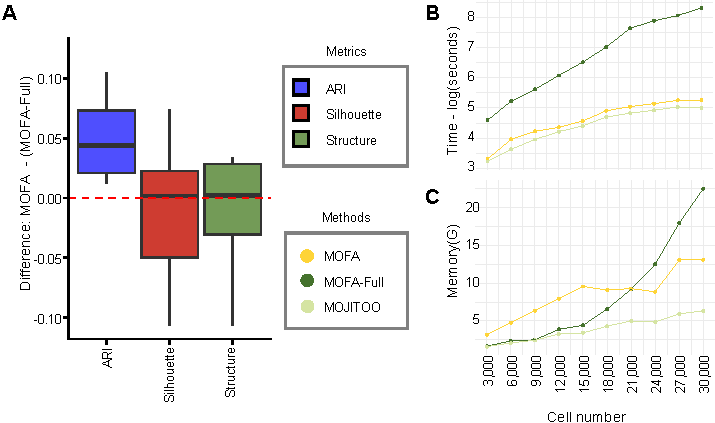
\includegraphics[width=0.95\textwidth]{MOFA/fig}
	\vspace{0.1cm}
	\caption[MOFA dimensional reduction comparison.]{\textbf{MOFA dimensional reduction comparison.} \textbf{A)} Boxplots shows differences MOFA with dimension reduction and with raw count matrix (MOFA-full) for ARI, Sihouette, Structure in all benchmarking datasets. The red dash line indicate the difference is equal to 0. \textbf{B)} Line plots showing elapsed time (log of seconds) for MOFA with dimension reductions input, MOFA-full with raw count matrix and MOJITOO (y-axis). \textbf{C)}Line plots showing peak memory(Gigabytes) required by MOFA with dimension reductions input, MOFA with raw count matrix and MOJITOO (y-axis). In both \textbf{B-C}, the x-axis shows the number of cells used (randomly sampled) from the \texttt{Skin-SHARE} data.}
	\label{fig:MOFA}
\end{figure}


\begin{figure}[!ht]
	\centering
	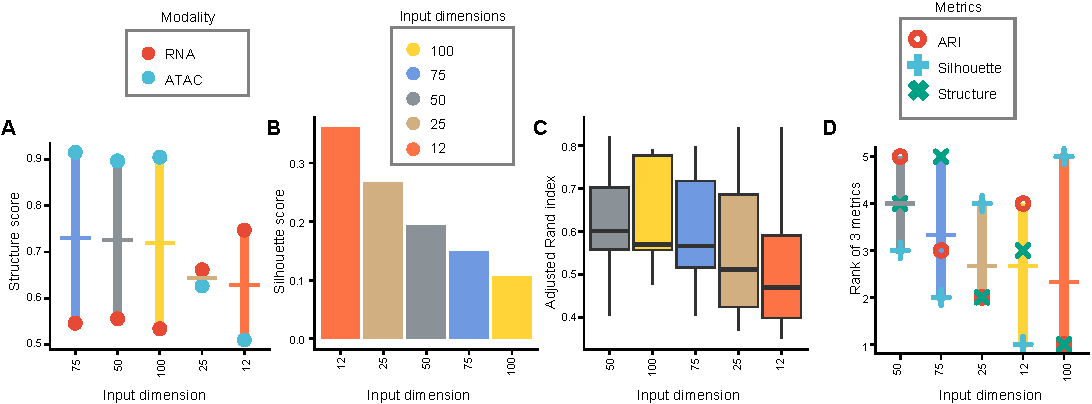
\includegraphics[width=0.95\textwidth]{Input_Dimensions/fig}
	\vspace{0.1cm}
	\caption[Input dimensions affection]{\textbf{MOJITOO applied to the PBMC-multiome data for distinct LSI and PCA dimensions.} \textbf{A)} We show the structure scores (y-axis) for distinct dimensions (x-axis). \textbf{B)} We show the Silhouete scores (y-axis) for distinct dimensions (x-axis). \textbf{C)} We show the distribution of Adjusted Rand score for distinct clustering results (resolution from 0.1 to 2.0) (y-axis) vs. number
of components (x-axis). \textbf{D)} We show the combined rank of the three previous metrics.}
	\label{fig:Input_Dimensions}
\end{figure}



\begin{figure}[!ht]
  \centering
  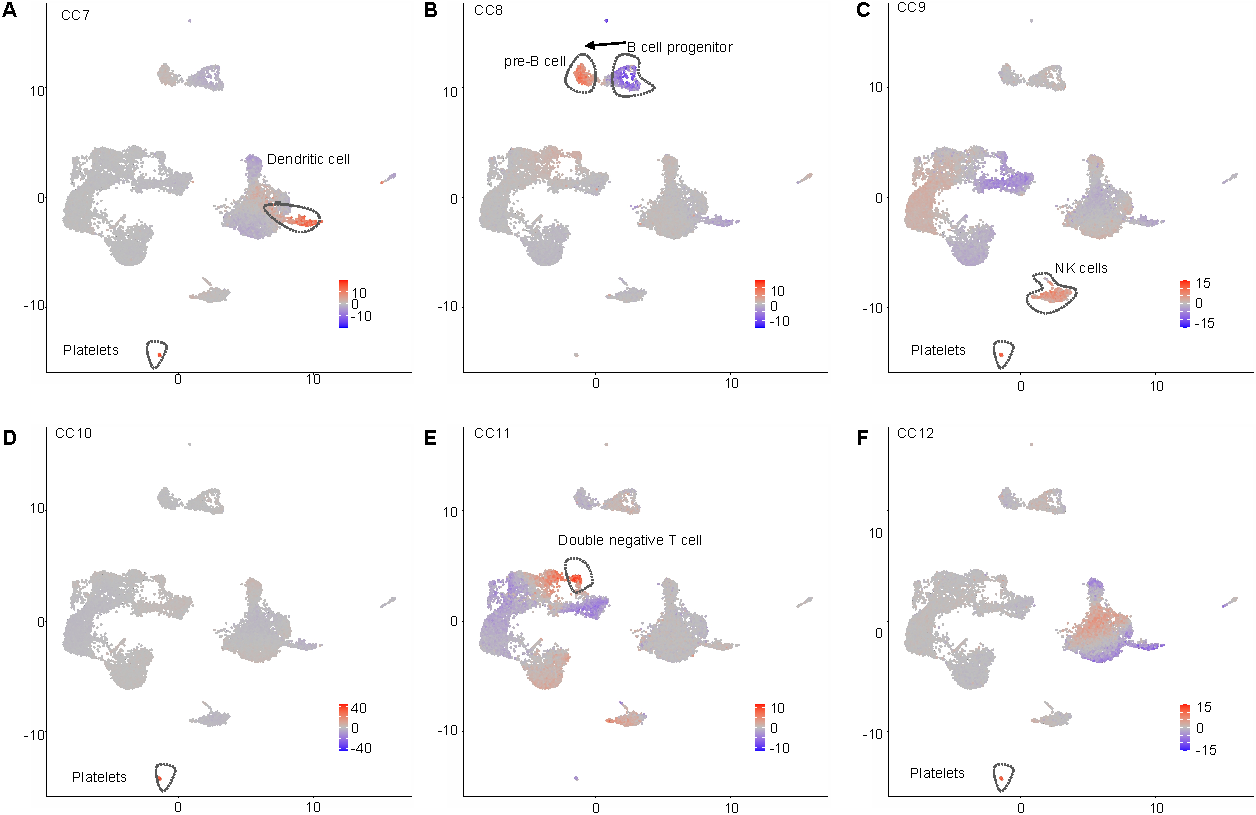
\includegraphics[width=0.95\textwidth]{Supp_CC_UMAP/fig}
  \vspace{0.1cm}
  \caption[PBMC CC7 to CC12 in UMAP]{\textbf{PBMC CC7 to CC12 in UMAP.} \textbf{A-F)}MAP with the scores of CC7 to CC12. We highlight major cell types associated to positive or negative CC scores and the arrow represents a potential differentiation process.}
  \label{fig:Supp_CC_UMAP}
\end{figure}


